\documentclass{article}

\usepackage{graphicx}
\usepackage{tikz}
\usepackage{tikzsymbols}
\usetikzlibrary{calc,patterns,shapes.geometric}
\pagestyle{empty}
\usepackage[margin=0pt]{geometry}
\geometry{papersize={14in,12in}}

\def\centerarc[#1](#2)(#3:#4:#5){\draw[#1] ($(#2)+({#5*cos(#3)},{#5*sin(#3)})$) arc (#3:#4:#5);}

\begin{document}
	\begin{figure}
		\centering
		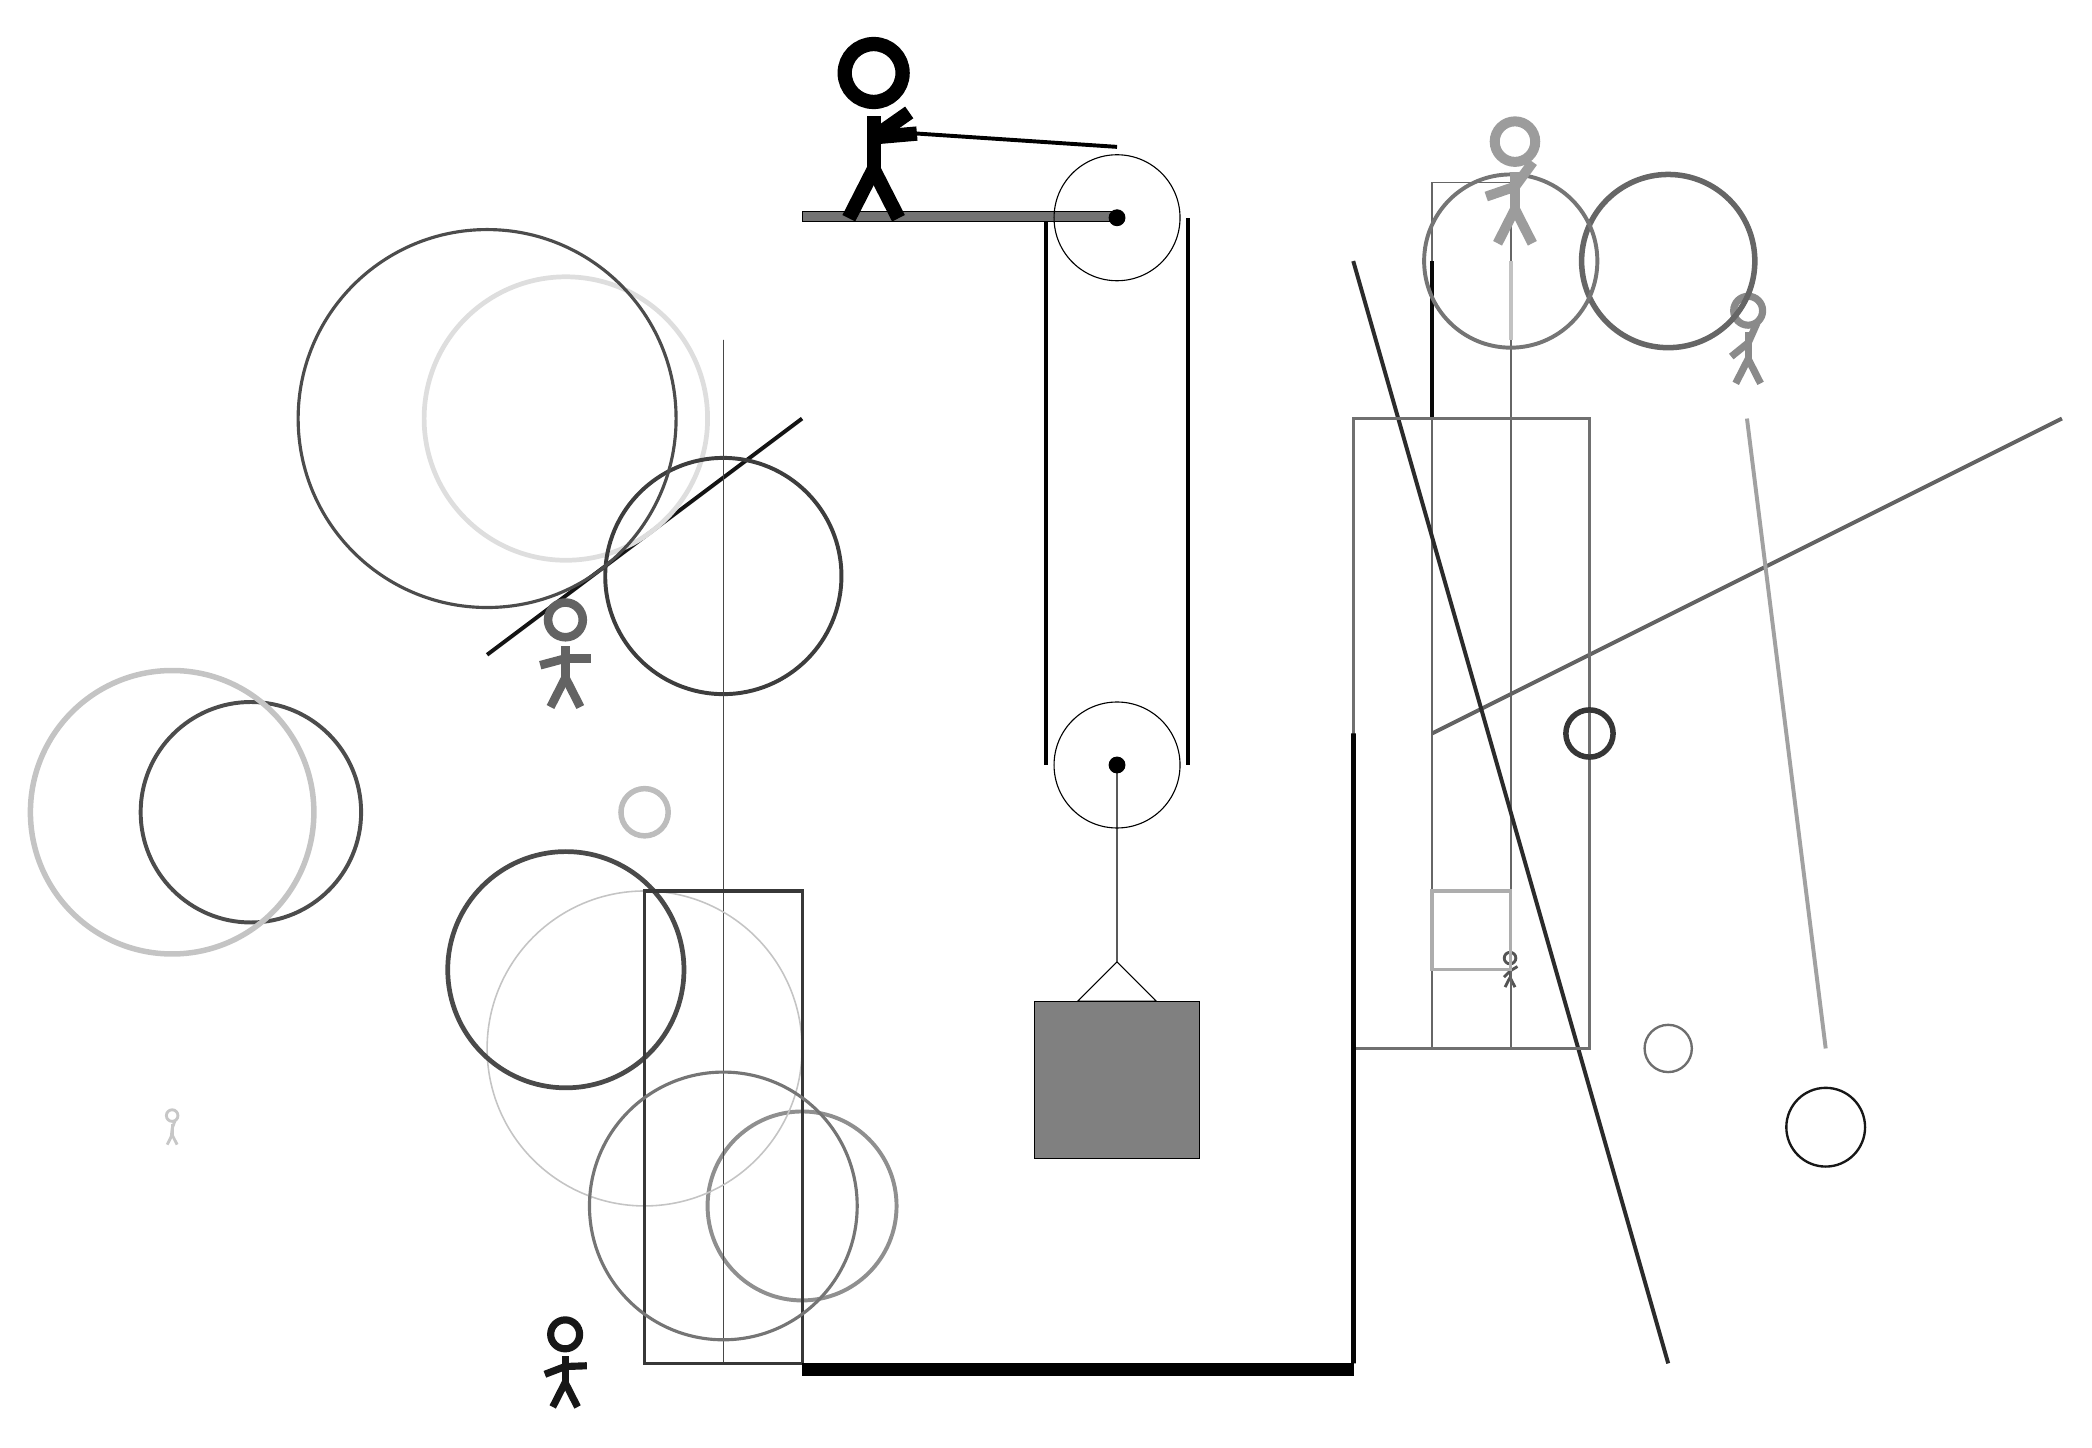
\begin{tikzpicture}
			%%%%% START %%%%%
			
			\draw[fill=black!55] (-2, 11.5) rectangle (2, 11.625);
			
			\draw (2, 4.6) circle (0.8);
			\draw[fill=black] (2, 4.6) circle (0.1);
			
			\draw (2, 11.55) circle (0.8);
			\draw[fill=black] (2, 11.55) circle (0.1);
			
			\draw (2, 4.6) -- (2, 2.1) -- (1.5, 1.6) -- (2.5, 1.6) -- (2, 2.1);
			\draw[fill=black!50] (0.95, 1.6) rectangle (3.05, -0.4);
			
			\draw[line width=0.5mm] (1.1, 11.5) -- (1.1, 4.6);
			\centerarc[line width=0.5mm](2, 4.6)(180:360:0.9);
			\draw[line width=0.5mm](2.9, 4.6) -- (2.9, 11.55);
			\centerarc[line width=0.5mm](2, 11.55)(0:90:0.9);
			\draw[line width=0.5mm](2, 12.45) -- (-1, 12.65);
			
			\draw [line width=0.5mm, color=black!70](-9, 4) circle (1.4);
			
			\node[line width=0.3mm, color=black!67] at (7, 2) {\Strichmaxerl[2][46][31]};
			\draw [line width=0.3mm, color=black!57](9, 1) circle (0.3);
			\draw[line width=0.5mm, color=black!92](-6, 6) -- (-2, 9);
			\draw [line width=0.5mm, color=black!44](-2, -1) circle (1.2);
			
			\draw [line width=0.6mm, color=black!13](-5, 9) circle (1.8);
			
			\node[line width=0.3mm, color=black!22] at (-10, 0) {\Strichmaxerl[2][84][70]};
			\node[line width=0.3mm, color=black!91] at (-5, -3) {\Strichmaxerl[5][21][2]};
			\draw [line width=0.5mm, color=black!76](-3, 7) circle (1.5);
			\draw[line width=0.2mm, color=black!60] (6, 12) rectangle (7, 1);
			
			\draw[line width=0.2mm, color=black!72] (-3, -3) rectangle (-3, 10);
			\draw [line width=0.2mm, color=black!23](-4, 1) circle (2.0);
			\draw[line width=0.5mm, color=black!61](6, 5) -- (14, 9);
			\draw [line width=0.3mm, color=black!91](11, 0) circle (0.5);
			\draw[line width=0.5mm, color=black!37](10, 9) -- (11, 1);
			\draw[line width=0.5mm, color=black!97](6, 11) -- (6, 9);
			\draw[line width=0.5mm, color=black!24](7, 10) -- (7, 11);
			\draw [line width=0.7mm, color=black!23](-10, 4) circle (1.8);
			\node[line width=0.4mm, color=black!61] at (-5, 6) {\Strichmaxerl[6][15][0]};
			\draw[line width=0.5mm, color=black!83](5, 11) -- (9, -3);
			\node[line width=0.3mm, color=black!46] at (10, 10) {\Strichmaxerl[5][39][66]};
			
			\draw [line width=0.6mm, color=black!71](-5, 2) circle (1.5);
			\draw[line width=0.4mm, color=black!56] (5, 1) rectangle (8, 9);
			\draw[line width=0.4mm, color=black!32] (6, 3) rectangle (7, 2);
			\draw [line width=0.4mm, color=black!70](-6, 9) circle (2.4);
			
			\draw [line width=0.7mm, color=black!60](9, 11) circle (1.1);
			
			\draw [line width=0.7mm, color=black!79](8, 5) circle (0.3);
			\draw[line width=0.4mm, color=black!78] (-4, 3) rectangle (-2, -3);
			
			\draw [line width=0.5mm, color=black!54](7, 11) circle (1.1);
			
			\draw [line width=0.7mm, color=black!26](-4, 4) circle (0.3);
			\draw[line width=0.6mm, color=black!98] (5, -3) rectangle (5, 5);
			
			\draw [line width=0.4mm, color=black!54](-3, -1) circle (1.7);
			\node[line width=0.5mm, color=black!39] at (7, 12) {\Strichmaxerl[7][19][54]};
			
			\node at (-1, 12.65) {\Strichmaxerl[10][-175][35]};
			
			\draw[fill=black] (-2, -3) rectangle (5, -3.15);
			
			%%%%% END %%%%%
		\end{tikzpicture}
	\end{figure}	
\end{document}